\documentclass[letterpaper, 12pt]{math}

\usepackage{amsmath}
\usepackage{pgfplots}
\pgfplotsset{compat=1.8}
\usetikzlibrary{arrows}

\title{Multivariable and Vector Calculus}
\author{Alvin Lin}
\date{August 2017 - December 2017}

\begin{document}

\maketitle

\section*{Cartesian Coordinates}
We take a standard x-y plane and put another axis perpendicular to it called
the z-plane and plot points as \( (x, y, z) \). This is known as the Cartesian
coordinate system.
\begin{center}
  \begin{tikzpicture}[x=0.2cm,y=0.2cm,z=0.2cm]
    \draw[->] (xyz cs:x=-13.5) -- (xyz cs:x=13.5) node[above] {$x$};
    \draw[->] (xyz cs:y=-13.5) -- (xyz cs:y=13.5) node[right] {$z$};
    \draw[->] (xyz cs:z=-13.5) -- (xyz cs:z=13.5) node[above] {$y$};

    \node[fill,circle,inner sep=1.5pt,label={below:\( (x_{1},y_{1},z_{1}) \)}]
      at (-3,-4,2) {};
    \node[fill,circle,inner sep=1.5pt,label={above:\( (x_{2},y_{2},z_{2}) \)}]
      at (3,5) {};
  \end{tikzpicture}
\end{center}

\noindent Cartesian Distance:
\[ d((x_{1}, y_{1}, z_{1}), (x_{2}, y_{2}, z_{2})) = \sqrt{
  (x_{2}-x_{1})^{2}+(y_{2}-y_{1})^{2}+(z_{2}-z_{1})^{2}} \]
Sphere of radius \( r \), center \( (x_{\circ},y_{\circ},z_{\circ}) \):
\[ (x-x_{\circ})^{2}+(y-y_{\circ})^{2}+(z-z_{\circ})^{2} = r^{2} \]

\subsection*{Example}
Give the largest sphere with center at \( (2,7,5) \) which fits within the I
octant \( (x>0,y>0,z>0) \).
\[ (x-2)^{2}+(y-7)^{2}+(z-5)^{2} = 2^{2} \]

\subsection*{Example}
\[ x^{2}+y^{2}+z^{2}-4x+2y-6z = 1 \]
What is the center and radius of such a circle?
\begin{align*}
  x^{2}-4x+y^{2}+2y+z^{2}-6z &= 1 \\
  x^{2}-4x+y^{2}+2y+z^{2}-6z &= 1 \\
  [(x-2^{2})-4]+[(y+1)^{2}-1]+[(z-3)^{2}-9] &= 1+4+1+9 \\
  (x-2)^{2}+(y+1)^{2}+(z-3)^{2} &= 15 \\
\end{align*}

\subsection*{Example}
Are the points \( P_{1}(1,2,3) \), \( P_{2}(2,3,4) \), \( P_{3}(0,2,6) \)
colinear?
\[ dist(P_{1},P_{2}) = \sqrt{3} \]
\[ dist(P_{2},P_{3}) = 3 \]
\[ dist(P_{1},P_{3}) = \sqrt{10} \]
Two of the distances should sum up to the third. This is not true for any of
these, thus the lines are not colinear.

\subsection*{Graphing in 3D}
Graph \( y = x^{2} \):
\begin{center}
  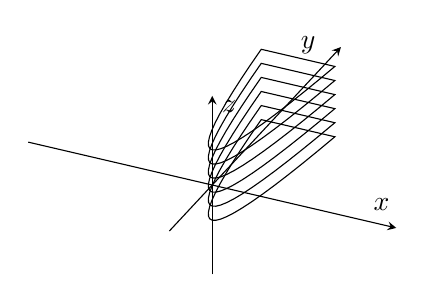
\begin{tikzpicture}
    \begin{axis}[
        axis equal,
        axis lines = center,
        xlabel = {$x$},
        ylabel = {$y$},
        zlabel = {$z$},
        enlargelimits = 0.5,
        ticks=none
    ]
      \addplot3[
          variable = \x,
          variable y = \y,
      ]({x}, {x^2}, {1});
      \addplot3[
          variable = \x,
          variable y = \y,
      ]({x}, {x^2}, {-1});
      \addplot3[
          variable = \x,
          variable y = \y,
      ]({x}, {x^2}, {3});
      \addplot3[
          variable = \x,
          variable y = \y,
      ]({x}, {x^2}, {-3});
      \addplot3[
          variable = \x,
          variable y = \y,
      ]({x}, {x^2}, {5});
      \addplot3[
          variable = \x,
          variable y = \y,
      ]({x}, {x^2}, {-5});
    \end{axis}
  \end{tikzpicture}
\end{center}
This graph extends up and down the z axis infinitely and form a surface.

\begin{center}
  If you have any questions, comments, or concerns, please contact me at
  alvin@omgimanerd.tech
\end{center}

\end{document}
